\renewcommand{\documentname}{Analysis}

\chapter{Analysis}

In this second chapter of software engineering, we will present the analysis conducted on the system to be built, with a brief general definition of what is intended to be done, recapitulating what was previously discussed in the theoretical sections.

The system requirements, both functional and non-functional, are also introduced, followed by an identification of the internal components of the system, the subsystems. An outline of class design is shown, focusing on the relationships between classes and data, which continues with an analysis of the identified use cases and the user interface. The chapter ends with a discussion of the tests to be carried out on the system.



\section{System definition}

The prototype defined in this document consists of a command line application which receives a list of text files as input and, by processing them, can perform three operations. The first and main one is the calculation of all the assignments required for the semester, starting from scratch or by using a previous list of assignments generated by the system itself. The second operation consists of finding holes in the schedule, that is, to find free classrooms which comply with a set of constraints. This is useful for assigning a class to a specific event even if the exact time or day of such an event is not known and can only be guessed. The last operation is the automation of the creation of the input files, which is done by converting some other files previously used by the School into new files which the system is able to process.



\section{System requirements}

The functional and non-functional requirements of the system. The non-functional requirements include the technological, system manuals and response time requirements.

\subsection{Functional requirements}

\begin{description}

    \item \textbf{RCLI} The system must implement a command line interface (CLI).
        \begin{description}
            \item \textbf{RCLI1} The CLI must show information about the current process being executed.
            \item \textbf{RCLI2} The CLI must show information about the GA.
                \begin{description}
                    \item \textbf{RCLI2.1} About the parameters of the GA.
                    \item \textbf{RCLI2.2} About the generations of the GA.
                    \item \textbf{RCLI2.3} About the execution time of the GA.
                \end{description}
            \item \textbf{RCLI3} The CLI must show information about the result of the execution.
                \begin{description}
                    \item \textbf{RCLI3.1} If the system terminated successfully.
                    \item \textbf{RCLI3.2} If the system terminated with errors, they will be also notified to the user.
                \end{description}
        \end{description}

    \item \textbf{RInput1} The system must receive the required data as input.
        \begin{description}
            \item \textbf{RInput1.1} The system must receive as input the classrooms of the School.
            \item \textbf{RInput1.2} The system must receive as input the groups of the semester.
            \item \textbf{RInput1.3} The system must receive as input the schedule of the groups.
            \item \textbf{RInput1.4} The system must receive as input the weeks in which the groups have classes.
            \item \textbf{RInput1.5} The system must receive as input the subjects of the semester.
            \item \textbf{RInput1.6} The system must receive as input the queries with the constraints for finding free classrooms in the schedule.
            \item \textbf{RInput1.7} The system must receive as input the previously used files for the automation of the system input files.
        \end{description}

    \item \textbf{RInput2} The system might receive optional data as input.
        \begin{description}
            \item \textbf{RInput2.1} The system might receive as input a total or partial list of assignments.
            \item \textbf{RInput2.2} The system might receive as input a list of classroom preferences.
            \item \textbf{RInput2.3} The system might receive as input a list of classroom restrictions.
        \end{description}

    \item \textbf{RInput3} The system must receive the required configuration files as input.
        \begin{description}
            \item \textbf{RInput3.1} The configuration files can be split into any number of files.
            \item \textbf{RInput3.2} The configuration files must include the information required by each functionality.
        \end{description}

    \item \textbf{RConf} The system must be configured by plain text files.
        \begin{description}
            \item \textbf{RConf1} System configuration must allow the user to control the parameters of the GA.
            \item \textbf{RConf2} System configuration must allow the user to specify the paths of the input files.
            \item \textbf{RConf3} System configuration must allow the user to specify the folder paths for the output files.
        \end{description}

    \item \textbf{RAssign} The system must perform the assignments by using AI algorithms.
        \begin{description}
            \item \textbf{RAssign1} The assignments should prioritise that Spanish and English groups go to different classes. 
            \item \textbf{RAssign2} The assignments may start from an initial set of assignments which must remain the same.
            \item \textbf{RAssign3} The assignments must maximize the number of groups of the same name and course assigned to the same theory classroom.
            \item \textbf{RAssign4} The assignments must maximize the number of groups of the same subject assigned to the same laboratory.
            \item \textbf{RAssign5} The assignments must leave a number of free laboratories in each time slot.
            \item \textbf{RAssign6} The assignments should prioritise that a laboratory does not end up with a large number of unused computers.
        \end{description}

    \item \textbf{RClassFinder} The system must be able to find free classrooms for an event given some constraints.
        \begin{description}
            \item \textbf{RClassFinder1} The constraints must include the date range for the search.
            \item \textbf{RClassFinder2} The constraints must include the range of hours for the search. 
            \item \textbf{RClassFinder3} The constraints must include the duration of the event (in hours) for the search.
            \item \textbf{RClassFinder4} The constraints must include the number of attendants to the event. 
            \item \textbf{RClassFinder5} The constraints must include the type of classroom to hold the event in. 
            \item \textbf{RClassFinder6} The constraints must include the maximum number of results to obtain. 
        \end{description}

    \item \textbf{RAutomation} The system must be able to automate the creation of the input files.
        \begin{description}
            \item \textbf{RAutomation1} The system must receive the planning for the semester.
            \item \textbf{RAutomation2} The system must receive the number of enrolled students for each group.
        \end{description}

    \item \textbf{RLog} The system must keep a log of its operations.
        \begin{description}
            \item \textbf{RLog1} The log must indicate the date and time of every record.
            \item \textbf{RLog2} The log must indicate the log level of every record.
            \item \textbf{RLog3} The log must record the complete information of encountered errors.
            \item \textbf{RLog4} The log must record basic information of the flow of the application.
        \end{description}

\end{description}


\subsection{Non-Functional requirements}

\begin{description}

    \item \textbf{RTech} The system requires a specific setup to be executed.
        \begin{description}
            \item \textbf{RTech1} The system requires Java 8 to be installed in the computer which executes it.
            \item \textbf{RTech2} The system requires that the folders where the input files are located have sufficient permissions for the system to be able to read these files.
        \end{description}

    \item \textbf{RMan} The system manuals must provide the readers with appropriate information for carrying out their tasks.  
        \begin{description}
            \item \textbf{RMan1} The installation manual must explain the setup needed before the execution of the program.
                \begin{description}
                    \item \textbf{RMan1.1} It is aimed both at the user and the developers of the application.
                \end{description}
            \item \textbf{RMan2} The execution manual must explain the syntax for executing each functionality of the system.
                \begin{description}
                    \item \textbf{RMan2.1} It is aimed both at the user and the developers of the application.
                \end{description}
            \item \textbf{RMan3} The user manual must explain all the functionality of the system.
                \begin{description}
                    \item \textbf{RMan3.1} It is aimed at the user of the application.
                    \item \textbf{RMan3.2} It must provide examples of usage with step by step instructions. 
                \end{description}
            \item \textbf{RMan4} The programmer manual must briefly explain the structure of the code and its components.
                \begin{description}
                    \item \textbf{RMan4.1} It is aimed at the developers and maintainers of the application.
                    \item \textbf{RMan4.2} It must provide examples of possible changes with some directions to implement them. 
                    \item \textbf{RMan4.3} It must provide an explanation on how to interpret the log of the application. 
                \end{description}
        \end{description}

    \item \textbf{RResponse} The system must perform the assignments of a semester in less than a day.
        \begin{description}
            \item \textbf{RResponse1} The assignments must have the expected quality. An assignment is said to be of quality if it meets all hard and as many soft constraints as possible.
        \end{description}

\end{description}



\section{Subsystem mapping}

In order to better understand the system, a study has been carried out on the subsystems that make up the system. The following subsystems have been identified:

\begin{itemize}

    \item \textbf{Algorithm subsystem:} Contains the greedy and genetic algorithms, as well as their operators and procedures.

    \item \textbf{Classfinder subsystem:} Contains functionality relating to the search for free classes in a time and schedule range.

    \item \textbf{Configuration subsystem:} Parses configuration files and keeps them in memory.

    \item \textbf{ErrorHandler subsystem:} It addresses the errors encountered and differentiates the expected from the unexpected.

    \item \textbf{Log subsystem:} It is in charge of creating and updating the system log.

    \item \textbf{Problem domain subsystem:} Defines the abstractions of the problem in the form of object types.

    \item \textbf{Central subsystem:} In charge of connecting the other subsystems to carry out the different functionalities of the system.

    \item \textbf{Persistence subsystem:} Responsible for parsing input files and constructing output files.

    \item \textbf{CLI subsystem:} Handles all text output to the console.

\end{itemize}




\section{Preliminary class diagram}


\begin{figure}[H]
    \caption{Preliminary class diagram}
  \centering
  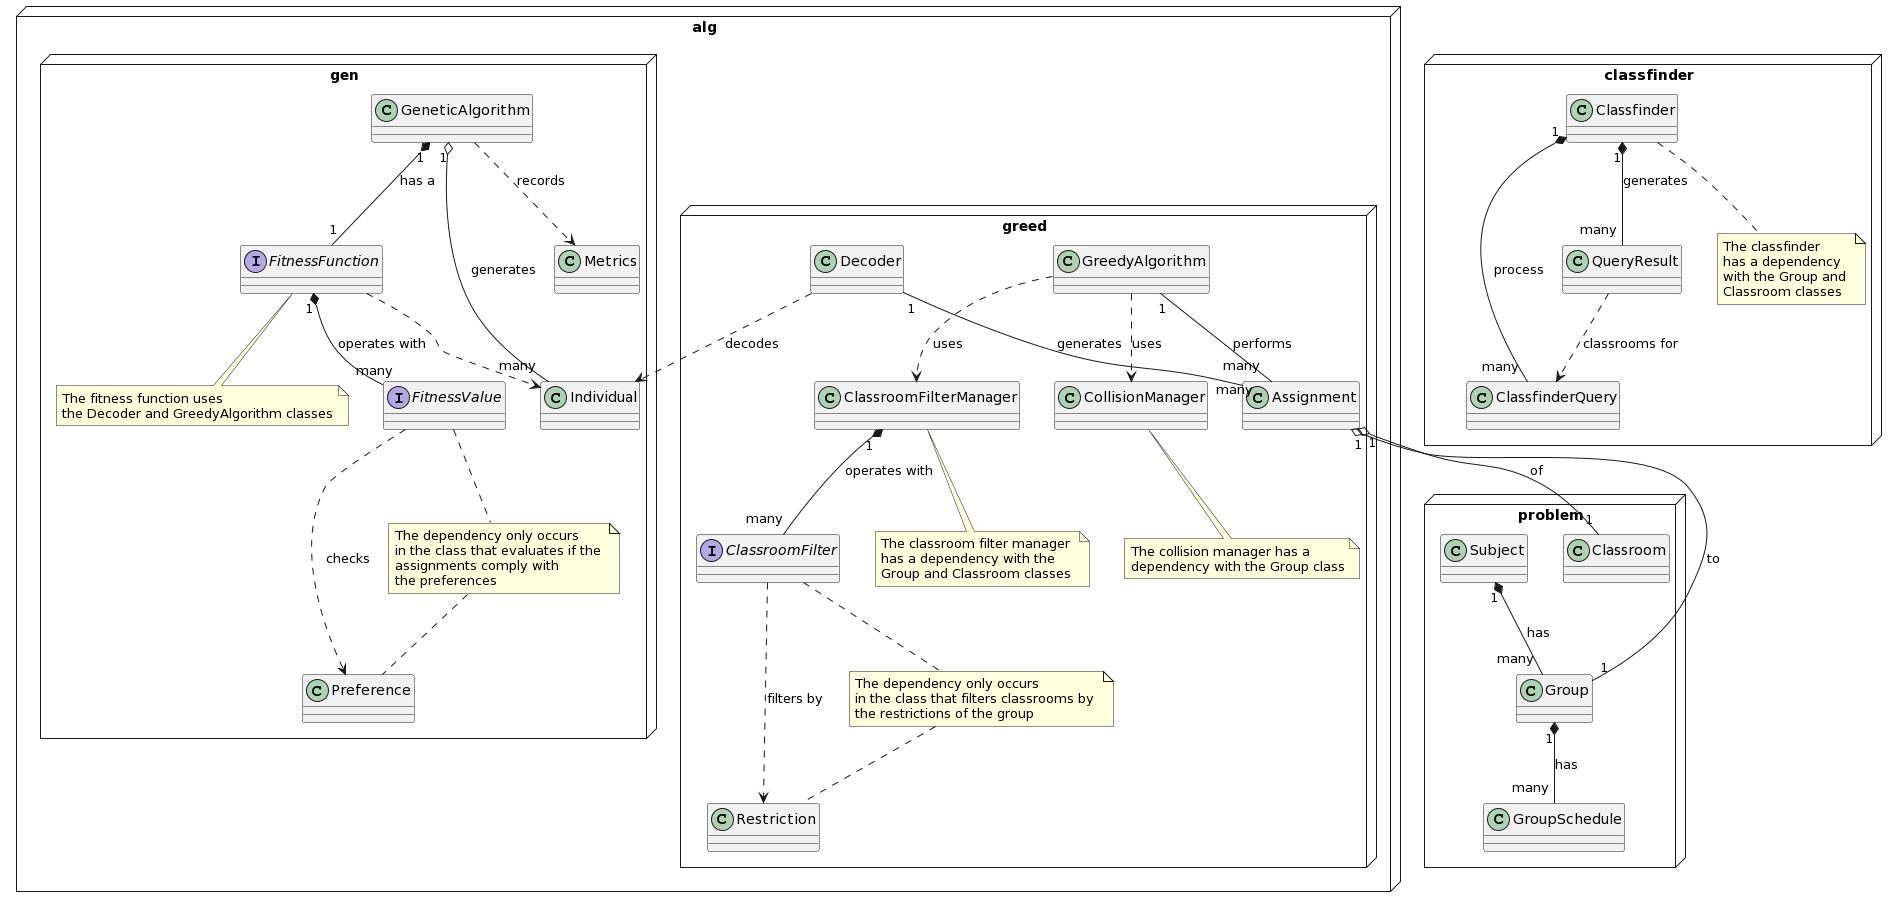
\includegraphics[scale=0.25]{initial_class_diagram_uml.png}
\end{figure}

Some notes on the previously shown class draft. It only contains classes from the business layer, because it is the most important part of the prototype.

The \textit{alg} package contains all classes related to the genetic and greedy algorithms. They are both interconnected by means of the fitness function of the GA, which uses the Decoder to get the assignments in the order specified by an individual and then calls the greedy algorithm with such a list of assignments. In the case of the greedy algorithm, some of its components, like the ClassroomFilterManager (which models the LFD) and the CollisionManager (which models the LCM) have a dependency with some classes of the problem domain package. That is also the case for the Assignment class, which represents an assignment of a classroom to a group.

The \textit{classfinder} package is a little more isolated than the alg package, but nevertheless has dependencies with some classes of the problem domain.

Finally, the \textit{problem} package models the problem domain, and contains the information of the abstracted models of the School and its environment. It is a key package not only for the different packages of the business layer, but also for the persistence layer, which depends on it for implementing the DataAccess to each abstraction.


\section{Analysis of use cases}

This section presents the analysis of the use cases of the system. Three use cases have been identified, each one reflecting a main functionality of the prototype. Therefore we have a use case for the assignment of classes to groups, the search for free classes by means of specific queries and the automatic generation of the system input files.

\begin{figure}[H]
    \caption{Use cases}
  \centering
  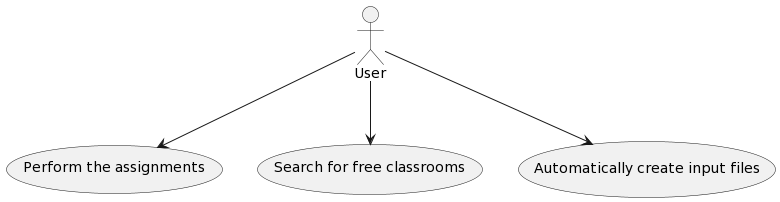
\includegraphics[scale=0.5]{use_cases_uml.png}
\end{figure}

For each use case, a table with information about the use case is presented. These tables contain the preconditions for the use case, the postconditions reached after its execution, a description of its steps, and a section with other variants of the use case. These tables are followed by a sequence and an activity diagrams, which will show the flow of the use case in a more visual way.

\subsection{Perform the assignments}

\begin{table}[H]
    \centering
    \caption{Use case description: Perform the assignments}
    \label{uc-table-assignments}
    \begin{tabular}{|p{4cm}|p{12cm}|}
        \hline
        \multicolumn{2}{|c|}{\textbf{PERFORM THE ASSIGNMENTS}} \\
        \hline
        \rowcolor{blue!10}
        \textbf{PRECONDITIONS} & \textit{The configuration files containing information about the GA and the input files need to be correctly formatted and must include the required data. Moreover, the input files with the classrooms, subjects, groups, group schedules, group academic weeks, restrictions, preferences and initial assignments must be correctly formatted.} \\
        \rowcolor{blue!30}
        \textbf{POSTCONDITIONS} & \textit{A text file with a report on the calculated assignments is generated. Also, a csv file with the assignments in the required format and a text file per classroom indicating its schedule in a timetable format are also written.} \\
        \rowcolor{blue!10}
        \textbf{DESCRIPTION} & 
        \textit{\begin{itemize}
                \item The user executes the program with the option flag signaling the calculation of the assignments and the path to the required configuration files.
                \item The system parses the configuration files. 
                \item The system parses the required and optional files indicated in the configuration files, as well as the GA parameters.
                \item The system executes the algorithms.
                \item The system outputs the best individual's information into a report text file, a csv file with the assignments and a text file for each classroom with its timetable.
            \end{itemize}
        } \\
        \rowcolor{blue!30}
        \textbf{SECONDARY SCENARIOS (VARIANTS)} & 
        \textit{\begin{description}
                \item \textbf{Variant 1. Errors on parsing.} If the system encounters any errors while parsing the input files, it will notify the user and store the information about such errors in the log file.
                \item \textbf{Variant 2. Not enough permissions.} If the system cannot read from or write into a folder because of insufficient permissions, it will notify the user and store the information about the error in the log file.
            \end{description}
        } \\
        \hline
    \end{tabular}
\end{table}


\begin{figure}[H]
    \caption{Sequence diagram: Perform the assignments}
  \centering
  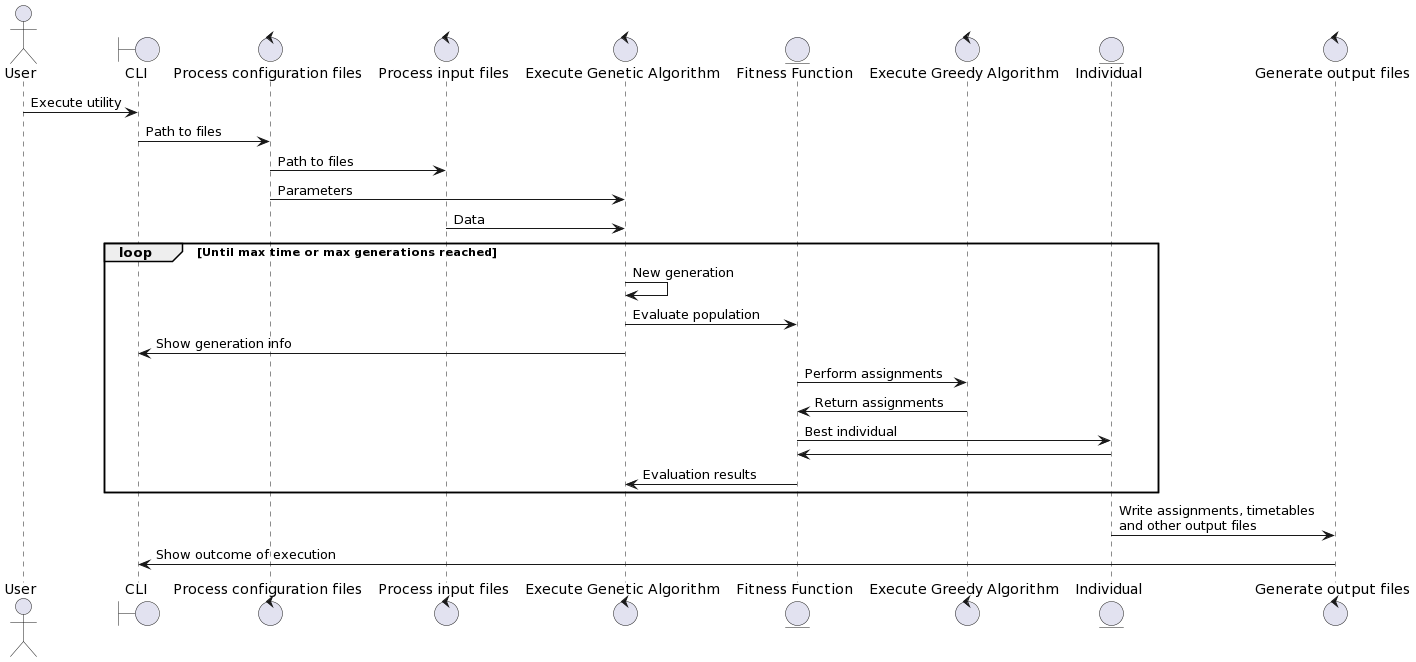
\includegraphics[scale=0.3]{uc_assignments_sequence_uml.png}
\end{figure}


\begin{figure}[H]
    \caption{Activity diagram: Perform the assignments}
  \centering
  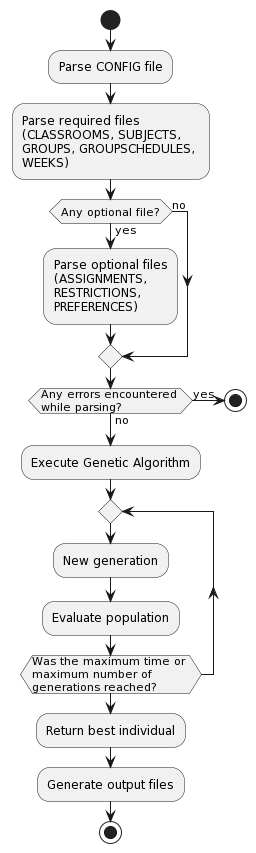
\includegraphics[scale=0.45]{uc_assignments_activity_uml.png}
\end{figure}




\subsection{Search for free classrooms}

\begin{table}[H]
    \centering
    \caption{Use case description: Search for free classrooms}
    \begin{tabular}{|p{4cm}|p{12cm}|}
        \hline
        \multicolumn{2}{|c|}{\textbf{SEARCH FOR FREE CLASSROOMS}} \\
        \hline
        \rowcolor{blue!10}
        \textbf{PRECONDITIONS} & \textit{The configuration files containing information about the input files needs to be correctly formatted and must include the required data. Moreover, the input files with the classrooms, subjects, groups, group schedules, group academic weeks, assignments and queries must be correctly formatted.} \\
        \rowcolor{blue!30}
        \textbf{POSTCONDITIONS} & \textit{A text file with the query results is generated.} \\
        \rowcolor{blue!10}
        \textbf{DESCRIPTION} & 
        \textit{\begin{itemize}
                \item The user executes the program with the option flag signaling the execution of the queries for finding free classrooms and the path to the required configuration files.
                \item The system parses the configuration files. 
                \item The system parses the required files indicated in the configuration files.
                \item The system executes the queries.
                \item The system outputs the result of all queries into a text file.
            \end{itemize}
        }\\
        \rowcolor{blue!30}
        \textbf{SECONDARY SCENARIOS (VARIANTS)} & \textit{Same as in \ref{uc-table-assignments}} \\
        \hline
    \end{tabular}
\end{table}


\begin{figure}[H]
    \caption{Sequence diagram: Search for free classrooms}
  \centering
  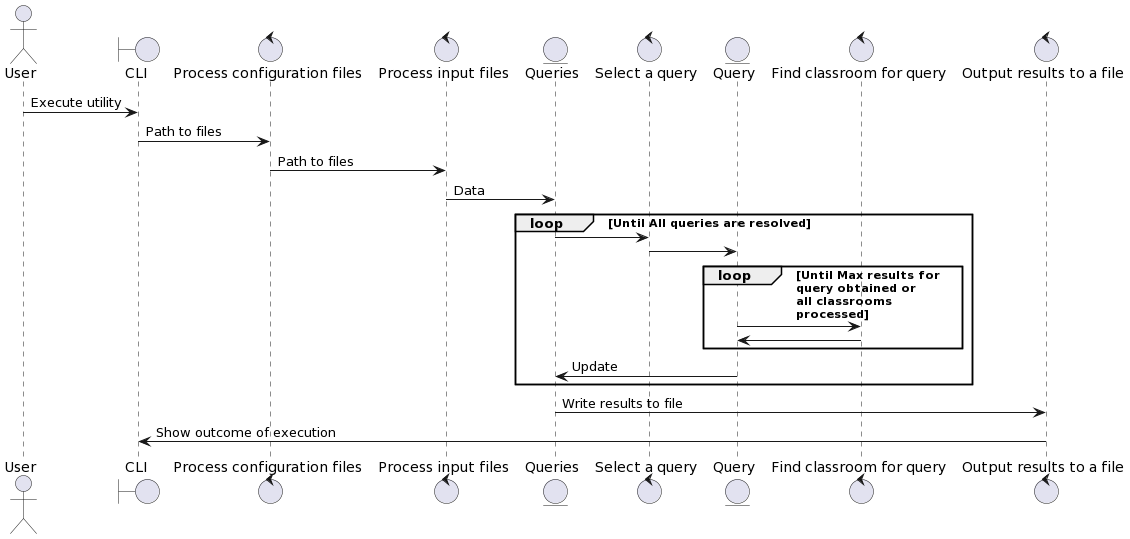
\includegraphics[scale=0.4]{uc_classfinder_sequence_uml.png}
\end{figure}


\begin{figure}[H]
    \caption{Activity diagram: Search for free classrooms}
  \centering
  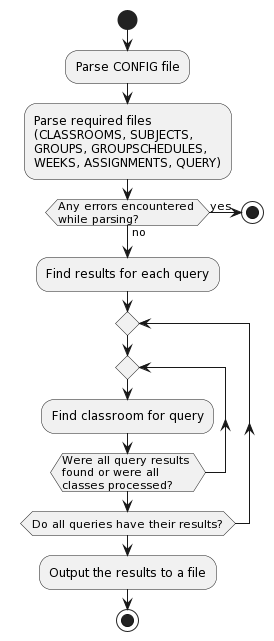
\includegraphics[scale=0.5]{uc_classfinder_activity_uml.png}
\end{figure}



\subsection{Automatically create input files}

\begin{table}[H]
    \centering
    \caption{Use case description: Automatically create input files}
    \begin{tabular}{|p{4cm}|p{12cm}|}
        \hline
        \multicolumn{2}{|c|}{\textbf{AUTOMATICALLY CREATE INPUT FILES}} \\
        \hline
        \rowcolor{blue!10}
        \textbf{PRECONDITIONS} & \textit{The configuration files containing information about the input files needs to be correctly formatted and must include the required data. Moreover, the input files with the planning for the semester and the number of enrolled students for each group must be correctly formatted.} \\
        \rowcolor{blue!30}
        \textbf{POSTCONDITIONS} & \textit{The files with the data of the subjects, groups, group schedules and group academic weeks are generated.} \\
        \rowcolor{blue!10}
        \textbf{DESCRIPTION} & 
        \textit{\begin{itemize}
                \item The user executes the program with the option flag signaling the generation of the input files and the path to the required configuration files.
                \item The system parses the configuration files. 
                \item The system parses the required files indicated in the configuration files.
                \item The system transforms the input files into the required format.
                \item The system outputs the result of each transformation in their own files.
            \end{itemize}
        }\\
        \rowcolor{blue!30}
        \textbf{SECONDARY SCENARIOS (VARIANTS)} & \textit{Same as in \ref{uc-table-assignments}} \\
        \hline
    \end{tabular}
\end{table}


\begin{figure}[H]
    \caption{Sequence diagram: Automatically create input files}
  \centering
  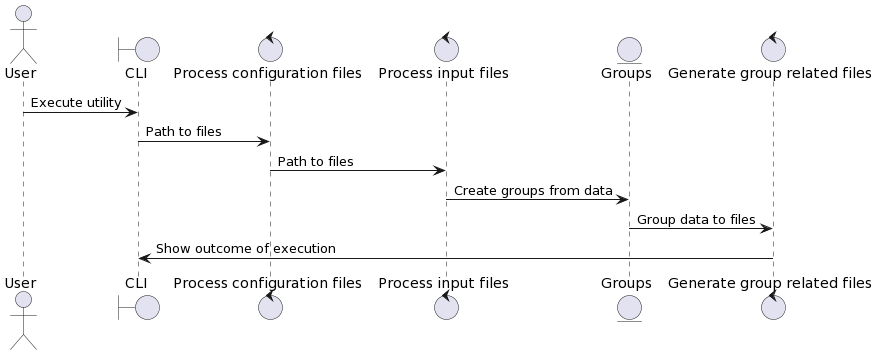
\includegraphics[scale=0.4]{uc_automation_sequence_uml.png}
\end{figure}


\begin{figure}[H]
    \caption{Activity diagram: Automatically create input files}
  \centering
  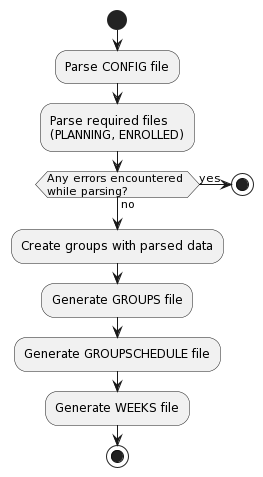
\includegraphics[scale=0.6]{uc_automation_activity_uml.png}
\end{figure}




\section{Analysis of user interfaces}

The prototype will have a Command Line Interface (CLI). The only interaction with the user occurs when they are calling the utility in the shell, indicating the option they want the prototype to execute and the necessary configuration files. As we explained before in the document, there are three main options for calling the prototype. One for performing the assignments, the second for finding free classrooms and the third for automating the creation of the input files.

Once the execution starts, the CLI will show relevant information to the user about the currently running processes (name and status). In the case of the GA execution, the selected parameters will be listed, as well as data on the results of each generation. The amount of information shown in the CLI about the GA can be controlled by the user through the configuration files. 



\section{Test plan specification}

Testing will focus on the parsing phase and the quality of the solutions obtained. In order to verify that both areas operate as expected, a battery of functional tests and an experimentation with various scenarios and instances will be carried out. Further details of the conducted experimentation are given in its own section (see Section \ref{experimental-results}), here we will focus on the test suite.


\begin{table}[H]
    \centering
    \caption{Test suite for UC: Perform the assignments}
    \label{uc-table-assignments}
    \begin{tabular}{|p{4cm}|p{8cm}|}
        \hline
        \multicolumn{2}{|c|}{\textbf{PERFORM THE ASSIGNMENTS}} \\
        \hline
        \textbf{Test} & \textbf{Expected result} \\
        \rowcolor{blue!30}
        No optional files & The assignment process will start from scratch and no restrictions or preferences are to be considered. \\
        \rowcolor{blue!10}
        Preferences & The assignment process will start from scratch and no restrictions are to be considered. Positive and negative preferences will be evaluated as soft constraints. \\
        \rowcolor{blue!30}
        Restrictions & The assignment process will start from scratch and no preferences are to be considered. Positive and negative restrictions will be evaluated as hard constraints. \\
        \rowcolor{blue!10}
        Partial assignments & The assignment process will start from the initial assignments and no preferences or restrictions are to be considered. The initial assignments will remain as they were once the allocation process is completed. \\
        \rowcolor{blue!30}
        All optional files & The assignment process will start from the initial assignments and the restrictions and preferences will be taken into account. \\
        \rowcolor{blue!10}
        Incorrect config format & The system will notify the error to the user. \\
        \rowcolor{blue!30}
        Incorrect input file format & The system will notify the error to the user. \\
        \rowcolor{blue!10}
        Incorrect input data & The system will notify the error to the user \\
        \hline
    \end{tabular}
\end{table}


\begin{table}[H]
    \centering
    \caption{Test suite for UC: Search for free classrooms}
    \label{uc-table-assignments}
    \begin{tabular}{|p{4cm}|p{8cm}|}
        \hline
        \multicolumn{2}{|c|}{\textbf{SEARCH FOR FREE CLASSROOMS}} \\
        \hline
        \textbf{Test} & \textbf{Expected result} \\
        \rowcolor{blue!30}
        Theory query & The system will look for theory classes that meet the requirements of the query. \\
        \rowcolor{blue!10}
        Lab query & The system will look for laboratories that meet the requirements of the query. \\
        \rowcolor{blue!30}
        Theory and lab query & The system will look for theory classes for one request and laboratories for the other. Each search must meet the requirements of its associated query. \\
        \rowcolor{blue!10}
        Incorrect config format & The system will notify the error to the user. \\
        \rowcolor{blue!30}
        Incorrect input file format & The system will notify the error to the user. \\
        \rowcolor{blue!10}
        Incorrect input data & The system will notify the error to the user \\
        \hline
    \end{tabular}
\end{table}


\begin{table}[H]
    \centering
    \caption{Test suite for UC: Automatically create input files}
    \label{uc-table-assignments}
    \begin{tabular}{|p{4cm}|p{8cm}|}
        \hline
        \multicolumn{2}{|c|}{\textbf{AUTOMATICALLY CREATE INPUT FILES}} \\
        \hline
        \textbf{Test} & \textbf{Expected result} \\
        \rowcolor{blue!30}
        Automation & The system will generate the input files necessary for the GA execution. \\
        \rowcolor{blue!10}
        Incorrect config format & The system will notify the error to the user. \\
        \rowcolor{blue!30}
        Incorrect input file format & The system will notify the error to the user. \\
        \rowcolor{blue!10}
        Incorrect input data & The system will notify the error to the user \\
        \hline
    \end{tabular}
\end{table}

